\pagebreak
\subsection{Mechanical Design} \label{Mechanical_Design}


\subsubsection{Structure}

The experiment consists on two cubic boxes, one stacked next to the other. The smallest box allocates the heaviest element, the CAC. The main box contains the AAC system as well as the general Electronic Box (EB). The frame of these two boxes will be made of aluminum bars which have a characteristic cross-section of 20x20 mm, see Figure \ref{cross-section}. The rails will allow an easy interface between bars and other elements. Bars will be joined together by using 90-degree angles, see Figure \ref{3_bars_joined}.

%% Cross section of one aluminum bar

\begin{figure}[!ht]
    \centering
    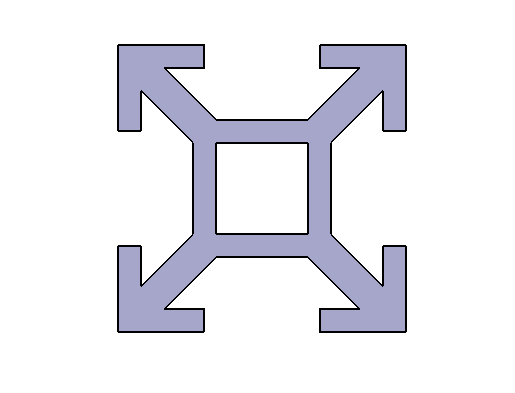
\includegraphics[width=0.5\textwidth]{4-experiment-design/img/1_cross_section.jpg}
    \caption{Cross section of the structural bars.}
    \label{cross-section}
\end{figure}

% Figure of 3 bars

\begin{figure}[!ht]
    \centering
    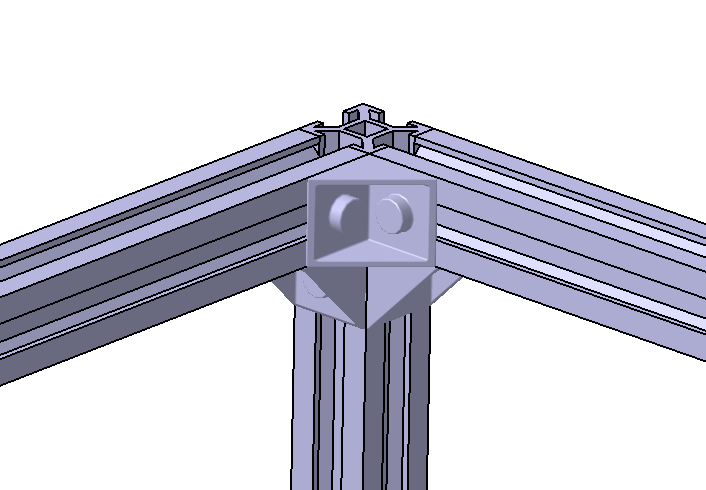
\includegraphics[width=0.6\textwidth]{4-experiment-design/img/bars_joint.jpg}
    \caption{Interface between structural bars.}
    \label{3_bars_joined}
\end{figure}

The frame is designed to withstand all vibrations and ensure a reliable stability of the entire system. Further tests will help to confirm and update the design if necessary. 

The two-box design will allow ease of access and manipulation of both the CAC and AAC subsystems, see Figure \ref{strucutre}. In addition, the AAC sampling system is designed to be re-usable for future handover to FMI, as such, it will be mountable on any standard balloon flight without having to introduce major design changes. The latter would imply to introduce a battery as a power unit, hence less bags could be carried (around 6 bags) in this potential future setup.

% Figure of the two structures one above the other one (slightly separated)
\begin{figure}[!ht]
    \centering
    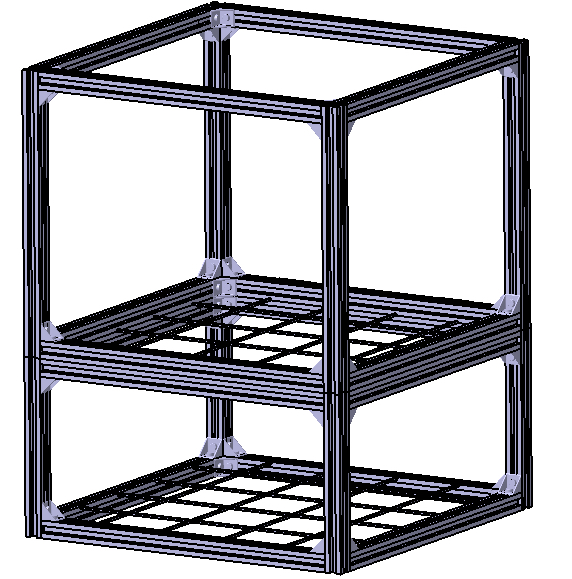
\includegraphics[width=0.7\textwidth, angle=90]{4-experiment-design/img/frame_structure.jpg}
    \caption{Structure of the two-box design.}
    \label{strucutre}
\end{figure}

\subsubsection{CAC Subsystem}

The CAC subsystem is designed with a 300-meter coiled tube, the valve governing it and a temperature sensor. To determine its positioning inside the gondola and the experiment box, some mechanical issues must be considered.

\smallskip
Firstly, it is possible to identify the interface to attach the experiment box to the gondola as one of the most critical points in terms of mechanics performance. In the worst case scenario, with a heavy experiment and without a proper study of the aforesaid interface, shear in the screws could be produced after a violent landing stress. Since the CAC will be the heaviest component in the whole experiment, its location and orientation will affect directly the stress analysis of the structure. The larger the distance to the fixed points, the bigger the Momentum produced by the component. Nevertheless, due to fast recovery implementation, the CAC tube will be placed vertically. Therefore, its dedicated box will be properly attached to the AAC box by means of 4 anchor points. The fast recovery then will only imply unscrewing 4 screws and disconnecting a wire. 

\smallskip
In order to command the valve, a wire will go out from the box and connected to the electronics interface panel located on an AAC box wall.

\smallskip
In addition, to avoid sample contamination with standstill air inside the gondola, the coil will have a direct outside inlet and outlet by means of an extension tube reaching further from the gondola’s limits.


\pagebreak
\subsubsection{AAC Subsystem}

The AAC Subsystem consists of 7 three-liter sampling bags. Each bag will have a dedicated valve in the Valve Center (VC) to allow emptying and filling processes as well as to close the bag when needed. The bags will be placed vertically and will have two anchor points: on the top through a  multiple anchor interface (see Figure \ref{anchor_bags}) and on the bottom by means of the tubes connecting them to the valves.

%% Several Figures of the top box with its inside elements: isometric, top view and front view.

\begin{figure}[!ht]
    \centering
    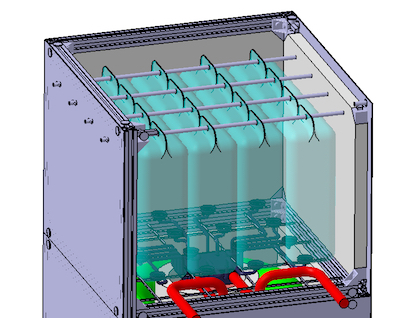
\includegraphics[width=0.7\textwidth]{4-experiment-design/img/anchored_bags.jpg}
    \caption{AAC Subsystem with all its elements.}
    \label{anchor_bags}
\end{figure}

\pagebreak
\subsubsection{Electronics Box}

The OBC and its external elements will be allocated in a bottom corner of the experiment box, inside AAC box, and on the opposite side of the CAC box. This will allow an easy access and manipulation as well as the required external interfaces. The smallest side of the EB will have the outer connections interfaces. Hence, the wall will have the necessary holes. The EB will be fixed to the AAC box structure bars in 3 different points.


%% Figure of the electronics box inside the coil, only bottom cube, isometric top view, explosion

%\begin{figure}[!ht]
 %   \centering
  %  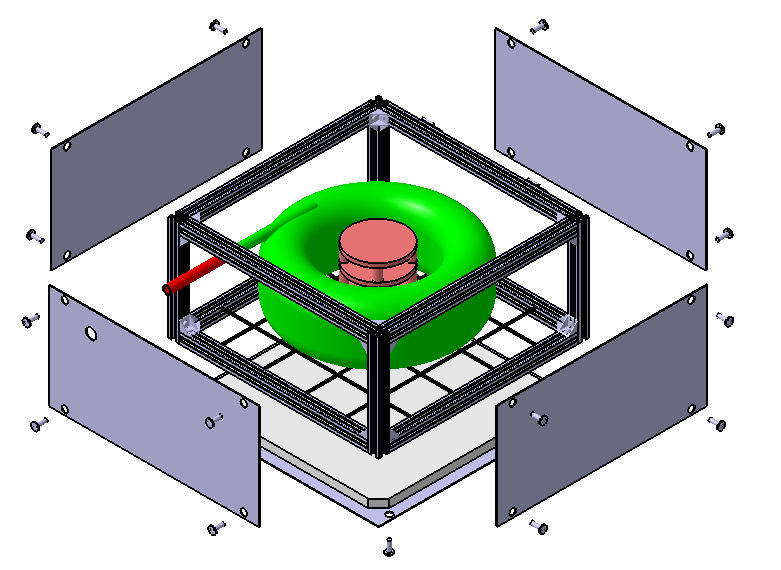
\includegraphics[width=0.7\textwidth]{4-experiment-design/img/explos_CAC.jpg}
   % \caption{.}
    %\label{electronics_box}
%\end{figure}

\pagebreak
\subsubsection{Valve Center}

The valve center consists of a coated box to which the AAC's 10 air sampling bags will be attached to. This box will serve as the air flow chamber. It will be connected to a pipe from which outside air will be pumped and also enable pre-sample collection flushing, see Figure \ref{valve_center_and_pipes}. The pump providing the airflow will be allocated on the inlet side and protected by an air filter. It will be allocated inside a shielding box, more detailed information in section \ref{Thermal_section}.

\smallskip
Both the pump box and the valve center will be allocated above the EB so all the command center is at the same place. Having them together will provide as well a proper cooling system monitored by several temperature sensors. A sketch of the setup can be seen in Figure ....

%% Figure of the valve center with the pipe and small tubes

%\begin{figure}[!ht]
%    \centering
%    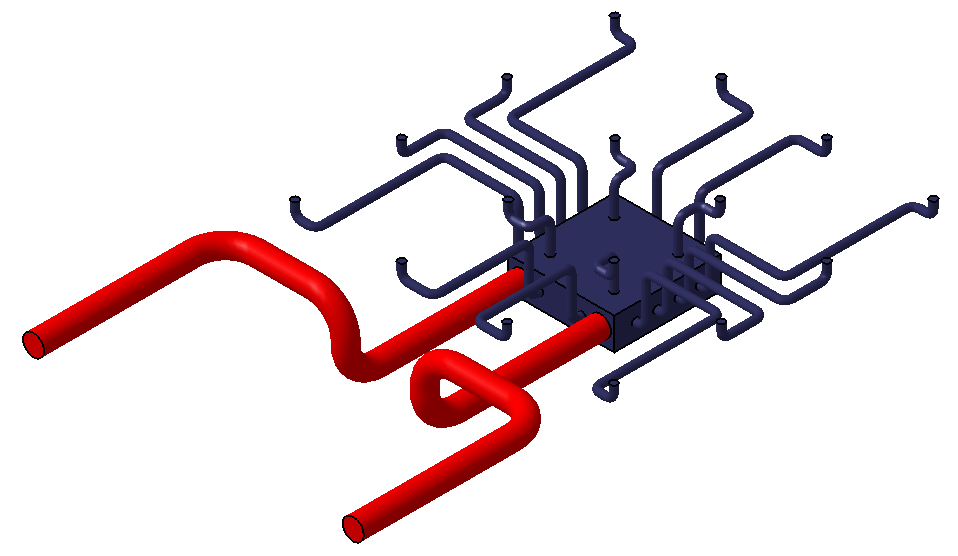
\includegraphics[width=0.9\textwidth]{4-experiment-design/img/valve_collector.jpg}
%    \caption{Valve center with all the tubes to the sampling bags and to the outside environment.}
%    \label{valve_center_and_pipes}
%\end{figure}

%% Add figure with EB and external interface + VC + Pump Box + Pipes + fixing elements

\pagebreak
\subsubsection{Protection}

In order to protect the components from all kind of external elements, the experiment box will be shielded with removable aluminum walls along with a thick layer of Styrofoam combined with Polyethylene foam attached to each wall. No internal space will be lost since the foam thickness is the same as that of the structural bars. Isolating sheets will also be glued in the walls to reinforce the temperature shielding. 
%Each box has an internal aluminum mesh at the bottom face. It will help to protect the CAC coiled tube from impacts as well as to withstand its considerable mass. On the other hand, the mesh in the upper box is used to fix the valve center at a privileged centered position.

The walls will properly protect both the CAC coiled tube and the AAC sampling bags from any external element, unexpected rapid movements, and a probable hard landing impact. Cross-section in Figure \ref{cut_all}. 


%% Cut: Figure CAC+EB, AAC+valve center, and walls + Styrofoam. Label all the parts

\begin{figure}[!ht]
    \centering
    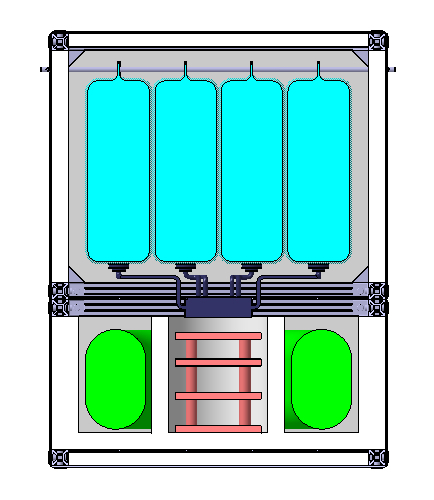
\includegraphics[width=0.7\textwidth]{4-experiment-design/img/tall_frontal.jpg}
    \caption{Cross-section of the whole experiment box.}
    \label{cut_all}
\end{figure}

The front walls, face of the experiment box exposed to the outside, will have several holes to allow the tubes providing air flow to collect clean air from the outside, see Figure \ref{front_wall_holes}.

%The top lateral walls will have four holes to allow the introduction of the circular bars used as anchor points for the sampling bags, see Figure \ref{anchor_bags}.

Bolts shall be used to attach all walls to the structure's railed bars.

%% Figure front wall holes: isometric Include labels

\begin{figure}[!ht]
    \centering
    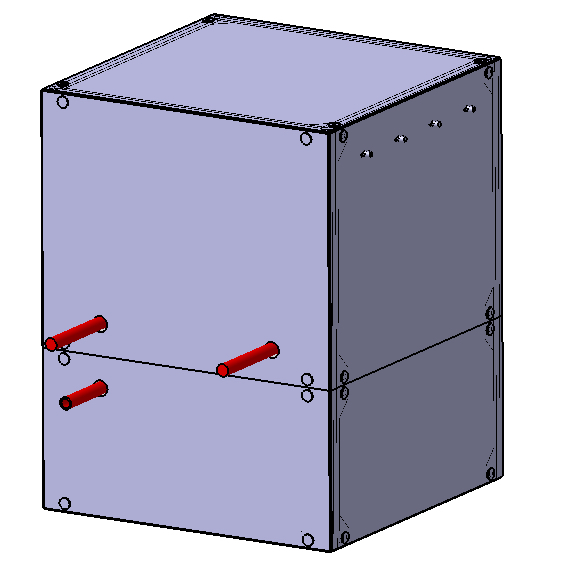
\includegraphics[width=0.7\textwidth]{4-experiment-design/img/frontal_holes.jpg}
    \caption{External view of the experiment.}
    \label{front_wall_holes}
\end{figure}

\pagebreak
\subsubsection{Fixing Interface}

The two experiment box subsystem structures will be joined together by four anchor points. On the front and back side, two flat plates with two bolts each will interface both structures. 

This method will allow for easy and fast recovery of the CAC box. 
 

%% Figure with the two boxes attached

\pagebreak
\subsubsection{Manipulation Interface}

The two-box system will be fixed to the gondola rails by using four 90-degree angles, 2 per rail. All the anchor points to the gondola will be in the AAC box since the CAC box will be already attached to it. The latter also ensures that the AAC box will remain properly fixed in the gondola after the CAC fast recovery. 

\smallskip
In order to access the experiment once fixed in the gondola, the walls could be removed when necessary providing access in all three directions. They can be screwed in again once the manipulation is done.


Several handles will be placed to allow an easy and safe manipulation of both the CAC and the AAC boxes. 


\subsubsection{Mechanical Components}

All the components used in the mechanical design can be found in Table \ref{tab:mechanical-components}. Spare elements are not included. 


\raggedbottom